\documentclass{beamer}

\usetheme{Madrid}

\usepackage[utf8]{inputenc}
\usepackage[frenchb]{babel}
\usepackage[T1]{fontenc}
\usepackage{amsmath}
\usepackage{hyperref}
\usepackage{comment} 
\usepackage{graphicx}
\usepackage[french]{algorithm2e}
\usepackage{alltt}

\usepackage{tikz}
\usetikzlibrary{arrows}

\pdfcompresslevel0
%%\renewcommand{\algorithmicforall}{\textbf{for each}}

\usepackage{color}
\usepackage{listings}

%% \addtobeamertemplate{footline}{\hfill\insertframenumber/\inserttotalframenumber}
  %% \hspace{10em}\\}

%% \addtobeamertemplate{footline}{\hfill\insertframenumber/\inserttotalframenumber}

\begin{document}

\setbeamertemplate{navigation symbols}{}

\title{Programmation générique basée sur les classes combinatoires}
\author{Marwan Ghanem - Charles Huyghues-Despointes}
\date{\today}

% slides number
\defbeamertemplate*{footline}{shadow theme}
{%
  \leavevmode%
  \hbox{
    \begin{beamercolorbox}[wd=.48\paperwidth,ht=2.5ex,dp=1.125ex,leftskip=.1cm plus1fil,rightskip=.1cm]{author in head/foot}%
    \usebeamerfont{author in head/foot}\insertframenumber\,/\,\inserttotalframenumber\hfill\insertshortauthor
  \end{beamercolorbox}%
  \begin{beamercolorbox}[wd=.5\paperwidth,ht=2.5ex,dp=1.125ex,leftskip=.1cm,rightskip=.1cm plus1fil]{}%
    \usebeamerfont{title in head/foot}\insertshorttitle%
  \end{beamercolorbox}}%
  \vskip0pt%
}

\beamertemplatenavigationsymbolsempty

\maketitle




\begin{frame}{Objectif}
\begin{itemize}
\item Definir un grammaire pour decrire les classe combinatoire.
\item Enrichir l'expressivité du grammaire (can we say it).
\item Représenter les classes ( structure arborescente ).
%%\item faire un lien entre les grammaires génératives et l'analyse combinatoire
\item Enumérer les objets par taille.
\end{itemize}

\end{frame}





\begin{frame}{Rappel de combinatoire analytique}
\begin{block}{Classe combinatoire}
Ensemble fini tel que : \\
\begin{itemize}
\item  On associe à chaque élément un nombre : sa taille.
\item La taille d'un élément est positive et finie.
\end{itemize}

On appellera Z la classe contenant un seul élément de taille 1.
\end{block}
\begin{exampleblock}{Les arbres binaires}
$\mathcal{B} = \mathcal{Z} + \mathcal{Z} \times \mathcal{B} \times \mathcal{B}$ \\
%%$\mathcal{Z}$ sert à dénombrer,ici on dénombre les feuilles, mais aussi les noeuds internes
Un arbre binaire est soit une feuille $\mathcal{Z}$ soit une un noeud avec deux arbres binaires ( $\mathcal{Z} \times \mathcal{B} \times \mathcal{B}$).
%%\item $ B = Leaf * <1> + B * B * <1> $\\
%%Séparation de ce qu'on compte et du terminal Leaf
\end{exampleblock}
\end{frame}



\begin{frame}{Vers un encodage des classes combinatoires }
Trouver une grammaire simple pour encoder les classes combinatoire. \newline
\begin{block}{Classe combinatoire}
\center
$\mathcal{M} = \mathcal{Z} + \mathcal{Z} \times \mathcal{M} \times \mathcal{M} + \mathcal{Z} \times \mathcal{M}$ \\  %%je modifie ici on avait mis * a place de times
\end{block}
\vspace{0.5cm}
\begin{block}{Notre grammaire}
\begin{alltt}
\center
M ::= Leaf * <1> + M * M * <1> + M * <1>;
\end{alltt}
\end{block}
\end{frame}




\begin{frame}{Vers un encodage des classes combinatoires NOT SURE OF THE TITLE}


\begin{block}{l’associativite <-1>}
\begin{figure}[h]
  \centering
  \includegraphics[scale=0.1]{1.png}
  $\Rightarrow$
  \includegraphics[scale=0.1]{2.png}
\end{figure}

\end{block}
\begin{block}{Expansion du Seq}
\begin{alltt}
B ::= Leaf * <1> + SEQ(B) * <1> ; \\
\end{alltt}
\vspace{0.2cm}
$\Rightarrow$
\begin{minipage}{0.7\textwidth}
\begin{alltt}
B ::= Leaf * <1> + D * <1>; \\
D ::= B * <0> + D * B <-1>;
\end{alltt}
\end{minipage}
\end{block}

%%\begin{itemize}
%%\item le produit commutatif
%%\item l'associativité ( < -1 > )
%%\end{itemize}
\end{frame}



\begin{frame}{Vers un encodage des classes combinatoires NOT SURE OF THE TITLE}


\begin{block}{Produit commutatif}
not sure what to say ?

\end{block}
\begin{block}{Expansion du Seq}
\begin{alltt}
B ::= Leaf * <1> + SET(B) * <1> ; \\
\end{alltt}
\vspace{0.2cm}
$\Rightarrow$
\begin{minipage}{0.7\textwidth}
\begin{alltt}
B ::= Leaf * <1> + D * <1>; \\
D::=B * <0> + B \& D * <-1>;
\end{alltt}
\end{minipage}
\end{block}
\end{frame}

\begin{frame}[fragile]{Algorithme I}
\begin{algorithm}[H]
  \KwIn{Grammaire deja parser et expansé (Composant)}
  \KwResult{Renvoie completeur}
  \ForAll{Composant}{
    \eIf{feuille de meme type exisit}{
       remplace le non terminaux par le feuille
    }{
     \eIf{Regle de meme type}{
      traite la regle.\\
      remplace le non terminaux par les arbres de cette regle.
      }{
        remplace le non terminaux par feuille non remplacable
      }
    }
  }
\end{algorithm}
\end{frame}
  %% \scalebox{0.8}[0.65]{
  %% \begin{algorithm}[H]
  %%  \KwResult{Genere tous les arbres de le taille demande}
  %%  addToTable(constructers)\;
  %%  start = 0\;
  %%  \While{true}{
  %%  List newList\;
  %%  List list = mainList.get(start)\;
  %%  taille = list.length\;
  %%  i = 0\;
  %%  sort(list)\;
  %%  \While{i < taille}{
  %%   Node tmp = list.get(i)\;
  %%   taille = tmp.getFils().length\;
  %%   \For{$j\leftarrow 0$ \KwTo $taille$}{
  %%     \For{$z\leftarrow 0$ \KwTo $constructers.length$}{
  %%      ArrayList <Node> t = tmp.AddLevel(constructers.get(z))\;
  %%      addList(t, newList)\;    
  %%     }
  %%   }
  %%   }
  %%   \eIf{newList.length == 0}{
  %%     break
  %%   }{
  %%   start++\;
  %%  }
  %% }
  %% \end{algorithm}
  %% }
%   \begin{verbatim}
% Entrée : une grammaire 
% Sortie : les constructeurs (noms non-terminaux)

% pour chaque SEQ et SET dans la grammaire
%   on fait l'expansion

% pour chaque nom non-terminal
%   on créé un nouveau nom terminal

% on renvoie tous les noms terminaux
% \end{verbatim}

% \begin{verbatim}
% Entrée :
% Sortie :

% On commence part une feuille
% on parcourt l'arbre, pour chaque feuille :
%   on complète la feuille
%   (2 cas + ou &)

% étape de rejet
% \end{verbatim}

\begin{frame}[fragile]{Algorithme II}
\begin{algorithm}[H]
  \KwIn{Liste de Completeur et la taille demande}
  \KwResult{Renvoie liste des arbres}
  \While{True}{
    \ForAll{Arbre de génération courant}{
      remplace une de ses feuille par un completeur\\
      \eIf{nouveau Arbre de taille  taille demande}{
         ajouter dans un nouveau génération
      }{rejeter l'arbre}
    }
    \eIf{nouveau génération est vide}{
      sortir du boucle
    }{
      continue
    }
    }
\end{algorithm}
\end{frame}

\begin{frame}{Exemple}
\textbf{Grammaire :} \\

\begin{alltt}
\hspace{10 mm} M::= Leaf * <1> + M * M * <1> + M * <1>;
\end{alltt}
\textbf{Completeur :} \\
\begin{figure}[h]
\centering
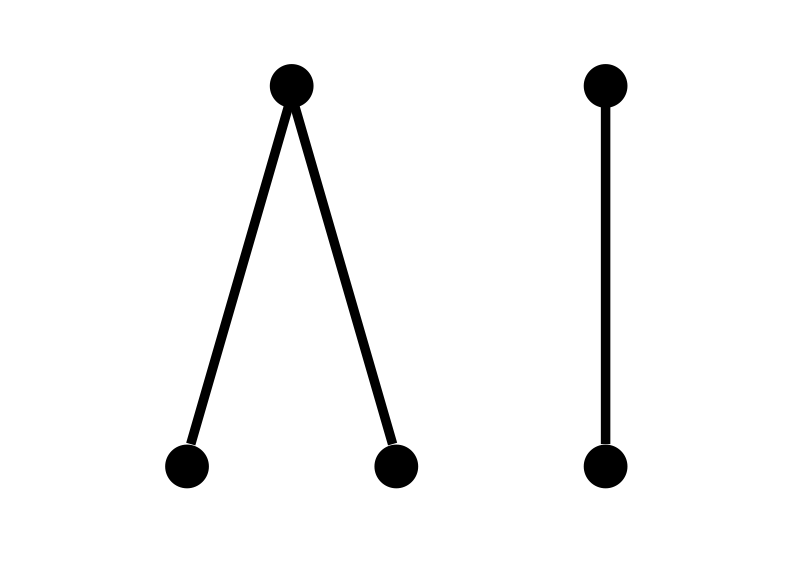
\includegraphics[scale=0.2]{const.png}
\end{figure}
\end{frame}


\begin{frame}{Exemple}
\textbf{Génération 1:}\\
\begin{itemize}
\item  Avec arbre unaire
\begin{figure}[h]
  \centering
  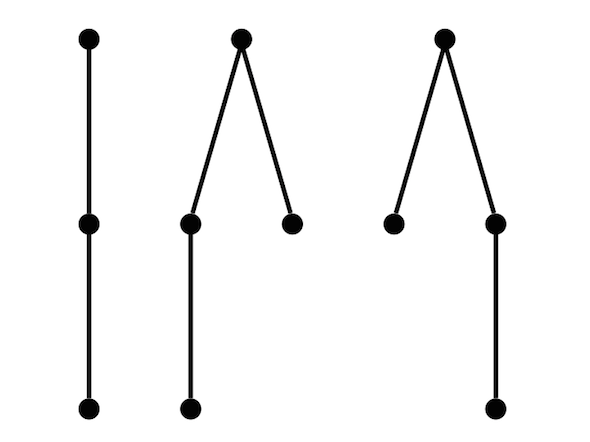
\includegraphics[scale=0.17]{gen1-1.png}
\end{figure}
\item Avec arbre binaire
\begin{figure}[h]
  \centering
  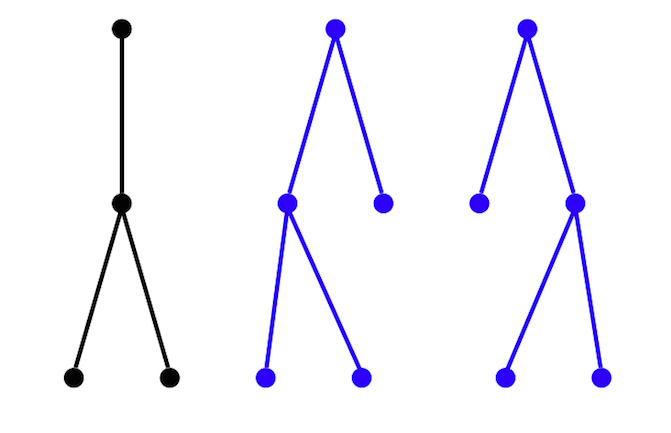
\includegraphics[scale=0.17]{gen1-2.png}
\end{figure}
\end{itemize}
\end{frame}



\begin{frame}{Exemple}
\textbf{Génération 2:}\\
\begin{itemize}
\item  Avec arbre unaire
\begin{figure}[h]
  \centering
  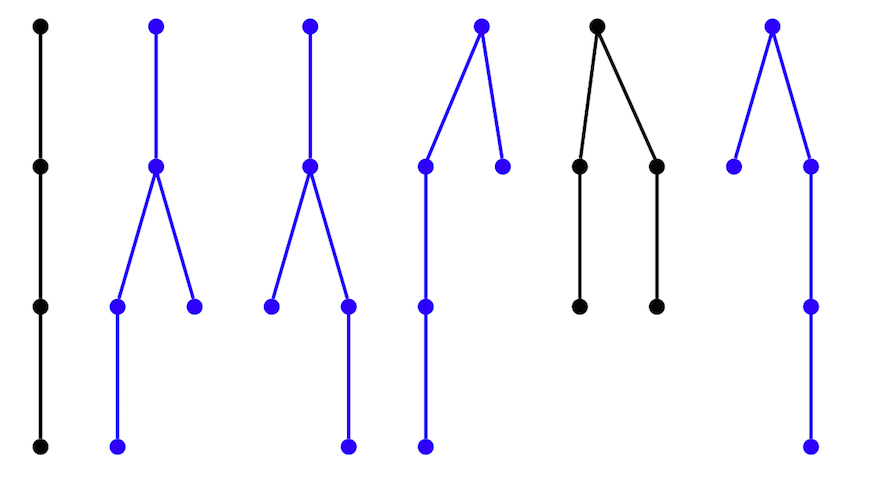
\includegraphics[scale=0.17]{gen2-1.png}
\end{figure}
\item Avec arbre binaire
\begin{figure}[h]
  \centering
  
\includegraphics[scale=0.17]{gen2-2.png}
\end{figure}
\end{itemize}
\end{frame}


\begin{frame}{Exemple}
\textbf{Génération 3:}\\
\begin{itemize}
\item  Avec arbre unaire
\begin{figure}[h]
  \centering
  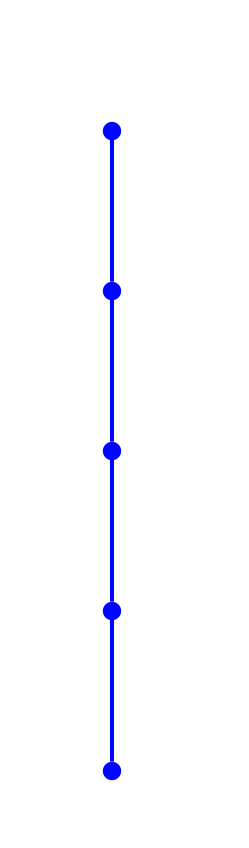
\includegraphics[scale=0.17]{gen3-1.png}
\end{figure}
\end{itemize}
\text{Nombre des arbres trouve au final : 9}
\end{frame}



\begin{frame}{Exemple: Partition et compostion d'entiers}
\begin{center}
\textbf{Composition et partition de 4} \\
\vspace{0.5cm}
\scalebox{1.2}{
\begin{tabular}{| c || c |}
\hline
Composition & Partation \\
\hline
1 + 1 + 1 + 1 & 1 + 1 + 1 + 1 \\ \hline
1 + 1 + 2 & 1 + 1 + 2 \\ \hline
1 + 2 +1 &   \\ \hline
2 + 1 + 1 & \\ \hline
2 + 2 & 2 + 2 \\ \hline
1 + 3 & 1 + 3 \\ \hline
3 + 1 & \\ \hline
4 & 4 \\ \hline
\end{tabular}
}
\end{center}
\end{frame}


\begin{frame}{Exemple: Partition et composition d'entiers}

\begin{block}{Composition :}
\begin{itemize}
\item Classe combinatoire :\\
\begin{alltt}
\hspace{10 mm} C = Seq(Seq$_{>0}$(Z)) \\
\end{alltt}
\item Notre grammaire : \\
\begin{alltt}
\hspace{10 mm} P ::= Leaf * <1> + SEQ(E) * <1>; \\
\hspace{10 mm} E ::= Leaf * <1> + SEQ(E) * <-1>; \\
\end{alltt}
\end{itemize} 
\end{block}

\end{frame}


\begin{frame}{Exemple: Partition et composition d'entiers}

\begin{block}{Partition :}
\begin{itemize}
\item Classe combinatoire :\\
\begin{alltt}
\hspace{10 mm} C = Set(Seq$_{>0}$(Z)) \\
\end{alltt}
\item Notre grammaire : \\
\begin{alltt}
\hspace{10 mm} P ::= Leaf * <1> + SET(E) * <1>; \\
\hspace{10 mm} E ::= Leaf * <1> + SEQ(E) * <-1>; \\
\end{alltt}
\end{itemize}
\end{block}
\end{frame}


\begin{frame}{Exemple: Partition et composition d'entiers}
\begin{figure}[h]
  \centering
  \includegraphics[scale=0.25]{partition4.png}
  \caption{Arbres des partitions de 4}
\end{figure}
\end{frame}

\begin{frame}{Bilan}
\begin{itemize}
\item Mise au point d'un langage de grammaire spécifique aux classes combinatoires.
\item Prise en charge des opérateurs d'union, produit, séquence et multi-ensemble.
\item Implémentation en Java ($\sim$ 3800 ligne). \\
  \footnotesize{\alltt{http://github.com/MarwanG/PSTL}}
\normalsize
\item Lien entre la combinatoire analytique et les grammaires génératives.
\end{itemize}
\end{frame}



\begin{frame}{Et après \ldots}
\begin{itemize}
\item Extension de la grammaire : PowerSet, Cycle, ... .
\item Génération automatique de code (fold, pattern matching...).
\item Problème de reconnaissance de forme.
\item Détection de grammaire ambigüe.
\end{itemize}
\end{frame}
\begin{frame}{Bibliographie}
  
  \begin{thebibliography}{9}
  \bibitem{Analytic}
    Philippe Flajolet et Robert Sedgewick
    \emph{ Analytic Combinatorics}.

  \bibitem{Analys}
    Philippe Flajolet et Robert Sedgewick
    \emph{An Introduction to the Analysis of Algorithms}.

  \end{thebibliography}

\end{frame}

\end{document}

